\documentclass[tikz,border=6pt]{standalone}
\usepackage{amsmath,amssymb,mathtools,physics,bm,nicefrac,wasysym}
\usepackage{xcolor}

\definecolor{colone}{RGB}{180,60,60}
\definecolor{coltwo}{RGB}{60,110,180}
\definecolor{colthree}{RGB}{60,140,80}

\definecolor{accent}{HTML}{A13D2C}
\definecolor{accent2}{HTML}{2B5F6B}
\definecolor{muted}{HTML}{5A564F}
\definecolor{panel}{HTML}{F8F6F0}
\definecolor{linecol}{HTML}{D8D2C4}
\definecolor{ink}{HTML}{1E1C1A}
\definecolor{astroblue}{HTML}{1B4F72}
\definecolor{astrodark}{HTML}{17202A}
\definecolor{sunyellow}{HTML}{E8A33D}

\usetikzlibrary{calc,arrows.meta,positioning,decorations.pathreplacing,decorations.markings,angles,quotes,shapes.geometric}
\usepackage{tikz-3dplot}

\newcommand{\vecr}{\vec r}
\newcommand{\vecL}{\vec L}
\newcommand{\vecA}{\vec A}
\newcommand{\vecf}{\vec f}
\newcommand{\vecF}{\vec F}
\newcommand{\vecp}{\vec p}
\newcommand{\avg}[1]{\left\langle #1\right\rangle}
\newcommand{\vecx}{\vec x}
\newcommand{\hatn}{\hat n}
\newcommand{\rhat}{\hat r}
\newcommand{\phihat}{\hat\phi}
\newcommand{\thetahat}{\hat\theta}
\newcommand{\note}[1]{\textcolor{blue!60!black}{\textit{[#1]}}}

% Astronomical acronyms
\newcommand{\LST}{\mathrm{LST}}
\newcommand{\GST}{\mathrm{GST}}
\newcommand{\GMST}{\mathrm{GMST}}
\newcommand{\GAST}{\mathrm{GAST}}
\newcommand{\LMST}{\mathrm{LMST}}
\newcommand{\LAST}{\mathrm{LAST}}
\newcommand{\UT}{\mathrm{UT}}
\newcommand{\UTC}{\mathrm{UTC}}
\newcommand{\TAI}{\mathrm{TAI}}
\newcommand{\TT}{\mathrm{TT}}
\newcommand{\TDB}{\mathrm{TDB}}
\newcommand{\JD}{\mathrm{JD}}
\newcommand{\MJD}{\mathrm{MJD}}
\newcommand{\EoT}{\mathrm{EoT}}
\newcommand{\SNR}{\mathrm{SNR}}
\newcommand{\RON}{\mathrm{RON}}

% Helper commands for specific diagrams
\newcommand{\midlinelabel}[3]{
    \node (midlabel) at ($ (#1)!.5!(#2) $) {#3};
    \draw[stealth-] (#1) --  (midlabel);
    \draw[-stealth] (midlabel) -- (#2);
}
\newcommand{\midlinelabell}[3]{
    \node[fill = white, inner sep = 0.2pt, outer sep=3pt] (midlabel) at ($ (#1)!.5!(#2) $) {#3};
    \draw[stealth-] (#1) --  (midlabel);
    \draw[-stealth] (midlabel) -- (#2);
}
\newcommand{\midlinelabelll}[3]{
    \node[fill = white, inner sep = 0.2pt, outer sep=3pt,scale=0.6] (midlabel) at ($ (#1)!.5!(#2) $) {#3};
    \draw[stealth-] (#1) --  (midlabel);
    \draw[-stealth] (midlabel) -- (#2);
}



\begin{document}
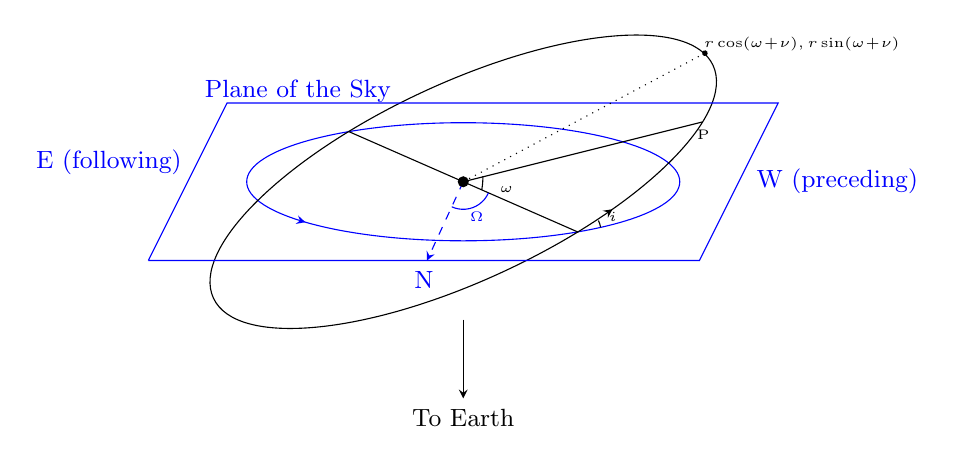
\begin{tikzpicture}
			\draw[blue,postaction={decorate,	decoration={markings,mark=at position 0.58 with {\arrow[>=stealth]{>}}}}] (0,0) ellipse (2.75 and 0.75);
			\draw[rotate=25,postaction={decorate,	decoration={markings,mark=at position 0.85 with {\arrow[>=stealth]{>}}}}] (0,0) ellipse (3.5 and 1.25);
			\draw [blue] (-4,-1)--(-3,1)--(4,1)--(3,-1)--(-4,-1);
			\draw (1.46,-0.64)--(-1.46,0.64);
			\draw (0,0)--(3.04,0.76);
			\draw [dashed,->,>=stealth,blue](0,0)--(-0.46,-1);
			\fill[black] (0,0) circle (2pt);
			\draw[->,>=stealth] (0,-1.75)--(0,-2.75);
			\draw [-{Circle[length=2pt]}, dotted] (0,0) -- (3.1, 1.65);
			\small
			\node at (0,-3) {To Earth};
			\node[blue] at (-0.5,-1.25) {N};
			\node[blue] at (-4.5,0.25) {E (following)};
			\node[blue] at (-2.1,1.15) {Plane of the Sky};
			\node[blue] at (4.75,0) {W (preceding)};
			\tiny
			\node at (4.3,1.75) {$r\cos(\omega\!+\!\nu), r\sin(\omega\!+\!\nu)$};
			\node at (3.05,0.6) {P};
			\draw (1.4,-0.64) ++(10:0.35) arc[start angle=10,end angle=25,radius=0.35];
			\node at (1.9,-0.45) {$i$};
			\node[black] at (0.55,-0.1) {$\omega$};
			\draw (0.25,0.07) arc [start angle=0, end angle=-10, radius=1];
			\draw[blue] (-114.7:0.35) arc[start angle=-114.7, end angle=-23.7, radius=0.35];
			\node[blue] at (-69.2:0.48) {$\Omega$};
		\end{tikzpicture}
\end{document}
